% !TeX program = pdflatex
%
% "A Retrieval-First Pipeline for Single-Image Global Geolocalization"
% Self-contained: compiles with pdflatex (two passes for cross-references).
% No external .bib file is required.
%
\documentclass[11pt,a4paper]{article}

\usepackage[utf8]{inputenc}
\usepackage[T1]{fontenc}
\usepackage{lmodern}
\usepackage[margin=1in]{geometry}
\usepackage{amsmath}
\usepackage{amssymb}
\usepackage{booktabs}
\usepackage{graphicx}
\usepackage{pgfplots}
\pgfplotsset{compat=1.18}
\usepackage{caption}
\usepackage{microtype}
\usepackage{xcolor}
\usepackage[colorlinks=true,linkcolor=black,citecolor=black,urlcolor=blue]{hyperref}
\usepackage{url}


\captionsetup{font=small,labelfont=bf}
\setlength{\parskip}{0.15em}

\title{\bfseries A Retrieval-First Pipeline for Single-Image Global\\
Geolocalization, and the Autonomous Ratchet That Found It}

\author{Josef Bednar\\
\small Independent researcher\\
\small \texttt{osobni@josefbednar.com}}

\date{July 2026}

\begin{document}
\maketitle

\begin{abstract}
\noindent
We describe a system that predicts the geographic coordinates of a single street-level
photograph with a median great-circle error of $34.1$~km on a frozen 2{,}998-image
validation set, and that runs entirely offline on a consumer Android phone. The system has
two stages. A DINOv3 ViT-L/16 backbone adapted with rank-16 LoRA classifies the image over
5{,}000 learned geocells; the resulting posterior gates a nearest-neighbour search over an
index of $1{,}198{,}072$ geotagged training images; a learned listwise reranker reorders the
top 100 candidates, and the winner's coordinates are returned verbatim. The classifier alone
reaches $104.7$~km. Everything below that number was bought for a few dollars of compute in
total, most of it spent on cached descriptors rather than on images.

Three findings drive the result. First, a geocell classifier is bounded by its own
quantization: with 5{,}000 cells and an argmax readout the median cannot fall below
$34.2$~km, and retrieval removes that bound by returning a real coordinate rather than a
cell centre. Second, the residual error is neither a data problem nor a gating problem: a
training image within 25~km exists for $100\%$ of validation queries and survives the gate
$92$ to $98\%$ of the time, yet the matcher selects one only $46\%$ of the time, so the
entire remaining gap is matching quality. Third, cheap post-hoc operations on cached
descriptors (hubness correction, whitening, multi-band contrastive heads and a
sixteen-feature logistic reranker) are collectively worth more than any of the encoder
fine-tunes we trained, and cost three orders of magnitude less.

The pipeline was found by an autonomous single-agent research loop that mutates one
experiment file, runs it once against a frozen evaluator, and keeps the change only if the
measured objective improves. We report the full ledger of 74 logged runs, including 35
rejected ideas and 9 crashes, and we treat the negative results as a primary contribution.
\end{abstract}

\section{Introduction}

Planet-scale image geolocalization asks a deceptively simple question: given one photograph
and nothing else, where on Earth was it taken? No metadata, no panorama, no user context.
The problem has been attacked in two broadly separate traditions. The retrieval tradition,
opened by IM2GPS \cite{hays2008im2gps} and revisited in the deep learning era
\cite{vo2017revisiting}, matches the query against a large geotagged database and transfers
the coordinates of the best match. The classification tradition, established by PlaNet
\cite{weyand2016planet} and refined by hierarchical and scene-aware variants
\cite{mullerbudack2018geolocation,clark2023where}, partitions the globe into cells and
trains a classifier over them. Recent work has largely converged on the classification
branch: PIGEON \cite{haas2024pigeon} builds semantically-aligned geocells and applies
haversine label smoothing, OpenStreetView-5M \cite{astruc2024osv5m} studies the
classify-then-regress hybrid at scale, and GeoCLIP \cite{cepeda2023geoclip} aligns image
features to a continuous location encoder.

This paper argues, from measurement rather than from principle, that at the accuracy levels
that matter for a practical product the classification branch is a means and the retrieval
branch is the end. A classifier is a good instrument for deciding \emph{where to look}. It
is a poor instrument for deciding \emph{exactly where}, because its output is quantized by
construction. Our classifier, trained on all $1.2$~M images of a Street View corpus for
three epochs, plateaus at a median error of $104.7$~km. The same frozen features, reused as
a retrieval index and searched under a posterior-mass gate, reach $78.5$~km on the first
attempt, and cheap post-processing on cached descriptors takes them to $42.7$~km without
ever touching an image again. Two short LoRA fine-tunes of the encoder and a
seventeen-parameter reranker carry the full pipeline to $34.1$~km.

The work has a second, methodological dimension that we do not think can be separated from
the first. Every experiment reported here was proposed, implemented, launched and scored by
an autonomous agent operating a keep-or-reset ratchet in the style of \cite{karpathy2026autoresearch}:
one experiment artifact is mutated, run once against a frozen evaluator, and kept only if the
objective improved. The human's role was to set the objective, to veto on grounds the metric
could not see, such as model size for a mobile target, and to sign off on spend. That regime
produced a specific and unusual research record: a complete ledger in which rejections are as
carefully documented as acceptances, because the agent needed them to avoid re-proposing dead
ideas. We report that ledger.

\paragraph{Contributions.}
\begin{enumerate}
\itemsep0.15em
\item A two-stage pipeline reaching a $34.1$~km median, $46.3\%$ within 25~km and $10.1\%$
within 1~km on a single static image with no metadata, scored by an evaluator that was
written before the study began and never modified during it.
\item A decomposition of the residual error into coverage ($100\%$), gate survival ($92$ to
$98\%$) and matcher selection ($46\%$), which identifies matching quality as the sole
remaining bottleneck and rules out three otherwise plausible directions.
\item A set of cheap techniques that run on cached vectors (band-wise geo-smooth
contrastive heads, candidate-side hubness correction, PCA whitening, and a sixteen-feature
listwise logistic reranker) and that take the frozen-feature index from $65.7$ to
$42.7$~km, and the final pipeline from $41.0$ to $34.1$~km, at approximately zero marginal
GPU cost.
\item An honest negative-results section covering thirty-five rejected ideas, including
several that improve every intermediate diagnostic while leaving the objective unchanged or
worse.
\item An on-device realization: the entire encoder and a $300$k-place index run offline on
an Android phone at $33.9$~km median, with a quantization study showing that int8 is
unusable for this backbone and why.
\end{enumerate}

\begin{figure}[t]
\centering
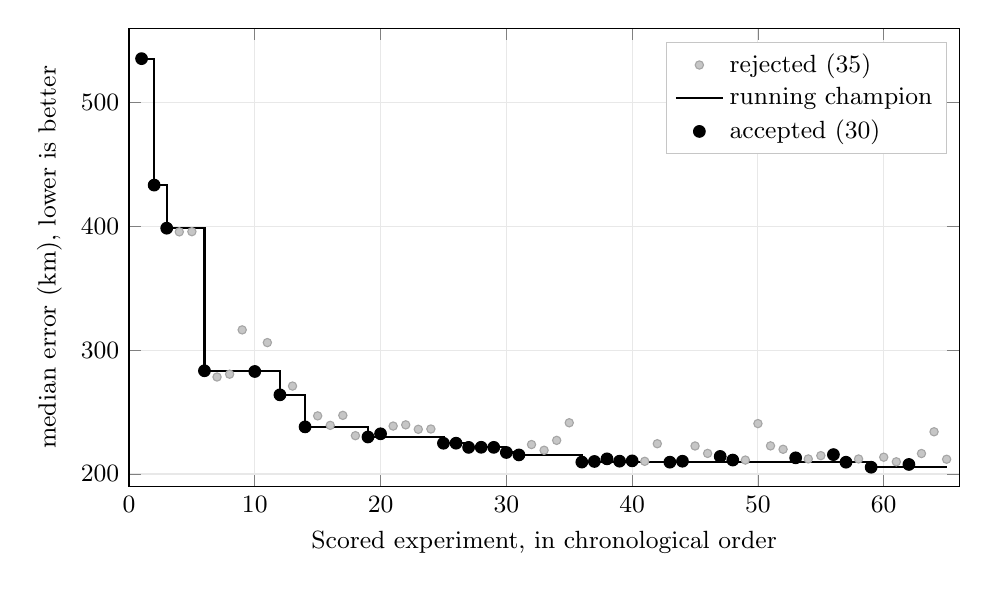
\begin{tikzpicture}
\begin{axis}[
  width=\textwidth, height=7.4cm,
  xlabel={Scored experiment, in chronological order},
  ylabel={median error (km), lower is better},
  xmin=0, xmax=66, ymin=190, ymax=560,
  grid=major, grid style={gray!18},
  tick label style={font=\small}, label style={font=\small},
  legend style={font=\small, draw=gray!45, fill=white, at={(0.985,0.97)}, anchor=north east},
  legend cell align=left,
]
\addplot[only marks, mark=*, mark size=1.5pt, draw=gray!70, fill=gray!45] coordinates {
(4,395.54) (5,395.70) (7,278.32) (8,280.59) (9,316.37) (11,306.11) (13,271.00)
(15,246.92) (16,239.27) (17,247.34) (18,230.93) (21,238.70) (22,239.67) (23,236.08)
(24,236.32) (32,223.77) (33,219.16) (34,227.15) (35,241.35) (41,210.22) (42,224.43)
(45,222.61) (46,216.62) (49,211.23) (50,240.69) (51,222.69) (52,219.94) (54,212.14)
(55,214.81) (58,212.11) (60,213.54) (61,209.85) (63,216.51) (64,234.08) (65,211.89)};
\addlegendentry{rejected (35)}
\addplot[const plot, thick, black] coordinates {
(1,535.43) (2,433.30) (3,398.49) (6,283.35) (12,263.90) (14,238.03)
(19,229.88) (25,224.80) (27,221.47) (30,217.35) (31,215.39)
(36,209.61) (43,209.53) (57,209.49) (59,205.46) (65,205.46)};
\addlegendentry{running champion}
\addplot[only marks, mark=*, mark size=2.1pt, black] coordinates {
(1,535.43) (2,433.30) (3,398.49) (6,283.35) (10,282.78) (12,263.90) (14,238.03)
(19,229.88) (20,232.45) (25,224.80) (26,224.85) (27,221.47) (28,221.56) (29,221.50)
(30,217.35) (31,215.39) (36,209.61) (37,210.11) (38,212.20) (39,210.34) (40,210.58)
(43,209.53) (44,210.30) (47,214.17) (48,211.23) (53,213.03) (56,215.65) (57,209.49)
(59,205.46) (62,207.69)};
\addlegendentry{accepted (30)}
\end{axis}
\end{tikzpicture}
\caption{The autonomous ratchet on the proxy objective (60{,}000 training images, an
eight-minute per-experiment budget, full 2{,}998-image validation split for scoring), plotted
directly from the committed run ledger. All 65 scored runs are shown; the 9 crashes are
omitted because they produce no number. The step function is the running champion,
$535.4 \rightarrow 205.5$~km. The accepted set includes re-runs of the champion used to
re-anchor after a change of rented machine, which is why some accepted points sit above the
champion line. A few rejected points sit below it: a gain smaller than the acceptance bar
of the moment was discarded as noise or held for a confirmation run, and the champion steps
on the confirmation. The named changes behind each step are listed in Table~\ref{tab:ratchet}. The
three largest single drops are a throughput change, a cell-count change and a change to the
prediction rule, in that order, and none of them is a change to the model architecture.}
\label{fig:ratchet}
\end{figure}

\section{Related work}

\paragraph{Classification over geocells.}
PlaNet \cite{weyand2016planet} framed geolocalization as classification over an adaptive
partition of the globe and established the template that most subsequent work follows.
Hierarchical variants \cite{mullerbudack2018geolocation} add coarse levels to catch
wrong-continent errors, and \cite{clark2023where} conditions on scene type. PIGEON
\cite{haas2024pigeon} contributes two ideas we adopt directly: geocells constructed to
respect administrative and semantic boundaries rather than pure density, and haversine label
smoothing, in which the target distribution over cells is $\mathrm{softmax}(-d/\tau)$ with
$d$ the great-circle distance from the true point to each cell centroid. We use $\tau = 75$~km
throughout, and an independent sweep over $\{40, 75, 110\}$~km confirmed that value as the
optimum for our cell count. PIGEON also reports that a retrieval refinement stage is
responsible for most of their sub-kilometre accuracy, which is consistent with what we
observe at much larger effect size.

\paragraph{Classify-then-regress.}
OpenStreetView-5M \cite{astruc2024osv5m} evaluates a broad design space and reports that
predicting a cell and then regressing a within-cell offset outperforms either alone. We
tried this twice, once as a per-cell tangent-plane regression head and once as a shared
offset head, and it failed both times at our training budget. The reason is instructive and
we return to it in Section~\ref{sec:negatives}: at a cell top-1 accuracy of $18\%$, the error
is dominated by choosing the wrong cell, not by position within the right one.

\paragraph{Visual place recognition.}
Once the problem is reframed as retrieval, the relevant literature is visual place
recognition. NetVLAD \cite{arandjelovic2016netvlad} and GeM pooling
\cite{radenovic2019finetuning} define the aggregation baseline; CosPlace
\cite{berton2022rethinking} and EigenPlaces \cite{berton2023eigenplaces} define the
large-scale training recipes; SALAD \cite{izquierdo2024salad} and BoQ
\cite{alibey2024boq} are the current descriptor state of the art. Patch-NetVLAD
\cite{hausler2021patchnetvlad} and its successors perform geometric verification of the top
candidates. Our failure mode, a Finnish forest road whose nearest neighbour is a
near-identical Finnish forest road 300~km away, is perceptual aliasing, which is a place
recognition problem rather than a geolocalization problem. That reframing was the most
productive single conceptual move of the project.

\paragraph{Retrieval post-processing.}
We use cross-domain similarity local scaling (CSLS) \cite{conneau2018word} to correct hubness
\cite{radovanovic2010hubs}, and PCA whitening \cite{jegou2012negative} on the raw descriptor
space. We evaluated and rejected $k$-reciprocal re-ranking \cite{zhong2017reranking}, graph
diffusion, and SuperGlobal-style query expansion \cite{shao2023superglobal}. Learned
reranking over a candidate set follows the Reranking Transformers line
\cite{tan2021instance}; our reranker is a much smaller model fit on a few thousand queries.

\paragraph{Backbones and adaptation.}
The encoder is DINOv3 ViT-L/16 \cite{simeoni2025dinov3}, the successor to DINOv2
\cite{oquab2024dinov2}, itself a Vision Transformer \cite{dosovitskiy2021image} with rotary
position embeddings \cite{su2024roformer}. We adapt it with LoRA \cite{hu2022lora} at rank 16
and never modify the pretrained weights. PatchDropout \cite{liu2023patchdropout} is used
during training only. Optimization is AdamW \cite{loshchilov2019decoupled}.

\paragraph{Concurrent work.}
Three recent papers surfaced during our own literature sweeps and influenced design choices
without being reimplemented in full: a semivariogram-based formulation of geographic hard
negative mining \cite{semivariogram2025}, HierLoc \cite{hierloc2026}, which embeds a
hierarchy of geographic entities in hyperbolic space, and Pinpoint \cite{pinpoint2026},
which reports a large gain from reranking on top of retrieval. The last of these was the
direct motivation for the reranker described in Section~\ref{sec:e7}.

\section{Task, data and evaluation protocol}

\subsection{Task}

One RGB image in, one $(\mathrm{lat}, \mathrm{lon})$ pair out. No panorama, no compass
heading, no capture time, no camera metadata, no text prompt. This is a deliberately
restrictive contract chosen because it is the contract a phone application can honour:
a user supplies a photograph and nothing else.

\subsection{Data}

We use \texttt{josefbednar/streetview-acw-300k}, a corpus of Street View panoramas sampled
worldwide. The training split contains $1{,}198{,}072$ images from $299{,}518$ distinct
locations at four headings each; the validation split alone spans 123 countries. The
held-out validation split contains $2{,}998$ images, each drawn from a distinct panorama
(verified by panorama identifier), so no validation image shares a location with another
validation image, and none shares a location with the training split. Sampling is pinned to
seed $1337$ and cached once, so every experiment in the program sees exactly the same
images.

For the fast experimental phase we use a frozen subset of $60{,}000$ training images
(approximately $15{,}000$ locations at four headings), and a fixed $1{,}000$-image
validation subset for in-training monitoring. Every reported score, including in that phase,
uses the full $2{,}998$-image split.

\subsection{Metrics}

The primary objective is the median great-circle error in kilometres, computed with the
haversine formula at $R = 6371.0088$~km. The median is chosen over the mean because the
error distribution has a heavy tail: roughly $2.5\%$ of images are sent to the wrong
continent, and those alone move the mean by hundreds of kilometres. We report the mean as a
secondary diagnostic and treat it, correctly, as a proxy for country-level accuracy rather
than for fine-grained precision.

Alongside the median we report $\mathrm{acc@}R$, the fraction of images within $R$
kilometres of the truth, at $R \in \{1, 25, 200, 750, 2500\}$~km, corresponding roughly to
street, city, region, country and continent resolution. We also report the GeoGuessr world
score, $5000 \cdot e^{-d/1492.7}$, because it is the metric a user of the deployed
application actually experiences. A rule of thumb worth keeping in mind throughout: a
proportion near $46\%$ measured on $2{,}998$ images carries a $95\%$ binomial interval of
roughly $\pm 1.8$ percentage points, so differences smaller than that between nearby
configurations should be read as suggestive rather than settled.

\subsection{The frozen harness}
\label{sec:harness}

Scoring lives in a separate module that was written before the study began and never
modified during it. It owns the data subset, the splits, the haversine implementation and
the metric panel. The model side exposes only a function mapping images to coordinates. The
experiment file was the only artifact allowed to change during the search, and this was
enforced structurally rather than by discipline: the launcher uploads only that one file to
the compute node, so the node keeps the original evaluator regardless of what the agent
edited locally. A score can therefore be improved only by making the model better, never by
making the test easier.

The harness also owns the training deadline. It arms a wall-clock alarm before the training
loop and raises an exception into the main thread at the budget, so every run terminates and
reaches its final evaluation even if it hangs. This detail matters more than it looks: it is
what makes an unattended overnight run produce a complete ledger rather than a partial
one.

\section{Methodology: an autonomous keep-or-reset ratchet}

\subsection{The loop}

The search procedure is a ratchet. An agent reads the accumulated research log, selects one
idea, edits the experiment file, runs it once on a rented GPU, parses the objective line from
the run output, and accepts the change only if it beat the current champion by more than the
noise floor. Rejected changes are reverted and recorded with the measured number and a short
diagnosis. There is exactly one experiment in flight at any time. There is no population, no
bandit, no surrogate model, and no parallel exploration. The only state carried
forward is the champion file and a written log.

The simplicity is the point. It makes the record auditable: every number in this paper
corresponds to one run of one file against one evaluator, and the file at that commit is in
version control.

\subsection{The proxy objective and its noise floor}

The full training corpus is too large to iterate on. The experimental phase therefore ran on
a proxy: $60{,}000$ training images and an eight-minute training budget per experiment,
scored on the full validation split. Two properties of this proxy were measured rather than
assumed.

Run-to-run variation on the proxy is $\pm 3$ to $5$~km on the median. We initially required a
gain of at least $8$~km before crowning a change, and later relaxed the rule to $1$~km with
no confirmation re-runs, on the human's instruction, after the acceptance rate collapsed. The
relaxation was a deliberate trade of precision for throughput and it is visible in the record:
several late-phase acceptances are within noise of each other.

More interesting, and less expected, is that the objective is not portable across rented
machines. The identical champion file, run on rented instances in different data centres,
scored $209.9$~km and $214.2$~km. Nothing about the model changed. We attribute this to
differences in achieved step count within the fixed wall-clock budget, and it forces a
protocol: after any machine change, re-run the champion to establish a local anchor, and
compare only against that anchor. Sessions that skipped this step produced comparisons we
later had to discard.

\subsection{What the ratchet found}

The proxy objective fell from $535.4$ to $205.5$~km, a reduction of $62\%$, across 74 logged
runs of which 30 were accepted (a figure that includes re-runs of the champion used as
baselines and machine anchors), 35 were rejected and 9 crashed. Figure~\ref{fig:ratchet}
shows the trajectory and Table~\ref{tab:ratchet} names every accepted change in order.

\begin{table}[t]
\centering
\footnotesize
\begin{tabular}{lrr}
\toprule
Accepted change & Median (km) & Anchor (km) \\
\midrule
Baseline: frozen DINOv3 ViT-L, LoRA $r{=}16$, 448~px, 512 geocells & 535.4 & \\
Remove gradient checkpointing, raise data-loader workers & 433.3 & \\
2048 geocells, average the top 16 & 398.5 & \\
Mode-seeking readout: temperature $0.5$, 1000~km locality & 283.4 & \\
Hierarchical heads at 64, 512 and 2048 cells & 263.9 & \\
Input resolution 448 to 384~px & 238.0 & \\
Fewer in-training evaluations & 229.9 & \\
Compile the backbone, warm up before the clock starts & 224.8 & \\
Larger real batch, made affordable by compilation & 221.5 & \\
Drop half the patch tokens in training forwards & 215.4 & \\
Double the batch again, spending the freed memory & 209.6 & \\
Country-level hierarchy with distance-smoothed targets & 209.5 & \\
Keep $60\%$ of patch tokens rather than $50\%$ & 213.0 & 214.2 \\
Median-seeking loss & 209.5 & 215.7 \\
Second, staggered tessellation & 205.5 & 215.7 \\
\bottomrule
\end{tabular}
\caption{Every accepted change, in the order it was accepted, with the proxy objective after
it. The last three rows were measured on different rented machines, where the champion itself
re-scores as shown in the anchor column; those rows are improvements against their own anchor,
not continuations of the column above them.}
\label{tab:ratchet}
\end{table}

The three largest single gains are worth naming, because none of them is an architectural
idea. Removing gradient checkpointing and raising the worker count bought $19\%$, because at
an eight-minute budget throughput is very nearly the objective. Growing the cell count from
512 to 2048 bought $8\%$, because the median was floored by cell size. Changing the
\emph{prediction rule} bought $29\%$, and is discussed in Section~\ref{sec:readout}.

The eleventh row is the most instructive of the set and Figure~\ref{fig:steps} shows why.
Dropping half the patch tokens in training doubled the number of optimizer steps that fit in
the budget, and the objective improved. Training at a lower resolution and evaluating at full
resolution raised the step count by $60\%$ again, to 4410, and the objective got \emph{worse}.
Doubling the batch instead cut the step count back to 1500 and produced the best result of the
whole phase. Step count is the currency only until roughly 2750 steps; past that point the
currency is per-step quality.

\begin{figure}[t]
\centering
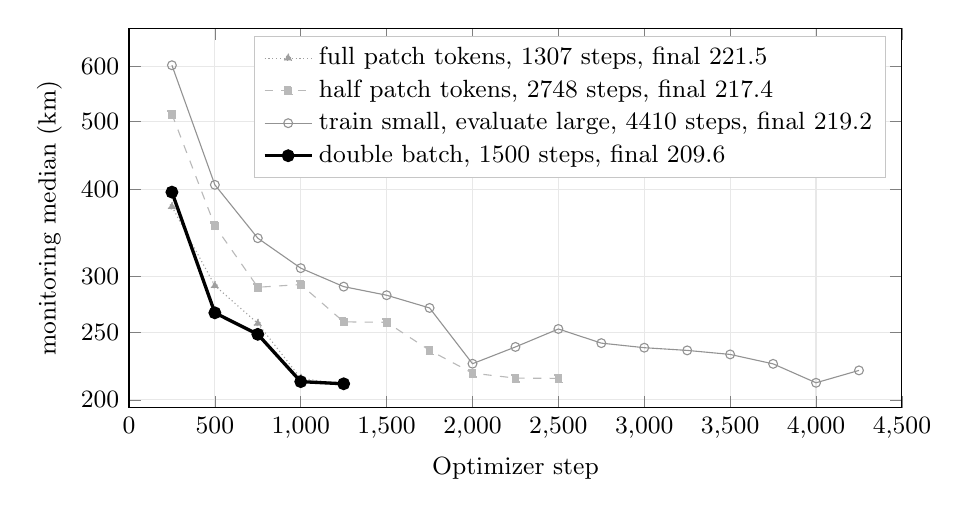
\begin{tikzpicture}
\begin{axis}[
  width=0.94\textwidth, height=6.4cm,
  xlabel={Optimizer step}, ylabel={monitoring median (km)},
  ymode=log, log ticks with fixed point,
  ytick={200,250,300,400,500,600}, yticklabels={200,250,300,400,500,600},
  xmin=0, xmax=4500, ymin=195, ymax=680,
  grid=major, grid style={gray!18},
  tick label style={font=\small}, label style={font=\small},
  legend style={font=\small, draw=gray!45, fill=white}, legend cell align=left,
]
\addplot[mark=triangle*, mark size=1.6pt, densely dotted, gray!75] coordinates {
(250,377.9) (500,291.3) (750,257.3) (1000,214.7) (1250,210.5)};
\addlegendentry{full patch tokens, 1307 steps, final 221.5}
\addplot[mark=square*, mark size=1.4pt, dashed, gray!55] coordinates {
(250,512.4) (500,354.7) (750,289.8) (1000,292.4) (1250,258.6) (1500,258.2)
(1750,235.5) (2000,218.4) (2250,214.9) (2500,214.7)};
\addlegendentry{half patch tokens, 2748 steps, final 217.4}
\addplot[mark=o, mark size=1.6pt, gray!85] coordinates {
(250,601.9) (500,406.0) (750,340.6) (1000,308.6) (1250,290.4) (1500,282.3)
(1750,270.7) (2000,225.3) (2250,238.1) (2500,252.6) (2750,241.1) (3000,237.5)
(3250,235.4) (3500,232.3) (3750,225.2) (4000,211.6) (4250,220.4)};
\addlegendentry{train small, evaluate large, 4410 steps, final 219.2}
\addplot[mark=*, mark size=1.7pt, very thick, black] coordinates {
(250,396.4) (500,266.4) (750,248.2) (1000,212.4) (1250,210.9)};
\addlegendentry{double batch, 1500 steps, final 209.6}
\end{axis}
\end{tikzpicture}
\caption{Step count stops being the currency. Curves are the in-training monitoring
evaluation on the fixed 1{,}000-image subset, logged live during four experiments that each
had the identical eight-minute budget; the number quoted in each legend entry is that run's
final score on the full validation split, which is the metric decisions were made on. The run
with the most steps by a wide margin is not the best, and the run with the fewest is. The
half-token run shown here is the first of its pair; its confirmation re-run scored
$215.4$~km, which is the figure that enters Table~\ref{tab:ratchet}.}
\label{fig:steps}
\end{figure}

\begin{figure}[t]
\centering
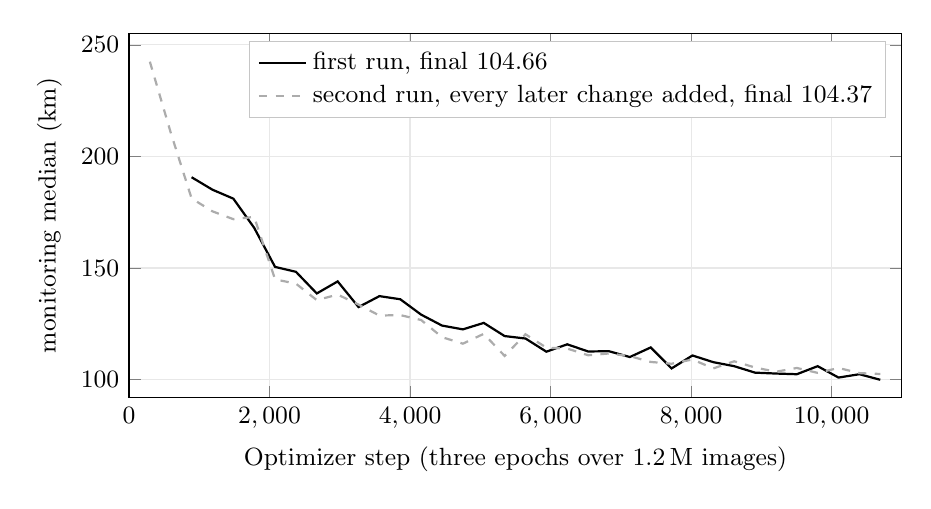
\begin{tikzpicture}
\begin{axis}[
  width=0.94\textwidth, height=6.2cm,
  xlabel={Optimizer step (three epochs over 1.2\,M images)},
  ylabel={monitoring median (km)},
  scaled x ticks=false, xtick={0,2000,4000,6000,8000,10000},
  xticklabel style={/pgf/number format/1000 sep={,}},
  xmin=0, xmax=11000, ymin=92, ymax=255,
  grid=major, grid style={gray!18},
  tick label style={font=\small}, label style={font=\small},
  legend style={font=\small, draw=gray!45, fill=white}, legend cell align=left,
]
\addplot[thick, black, mark=none] coordinates {
(891,190.7) (1188,185.1) (1485,181.1) (1782,168.0) (2079,150.5) (2376,148.3) (2673,138.6)
(2970,144.0) (3267,132.5) (3564,137.4) (3861,136.0) (4158,129.1) (4455,124.2) (4752,122.5)
(5049,125.4) (5346,119.5) (5643,118.4) (5940,112.5) (6237,115.8) (6534,112.6) (6831,112.7)
(7128,110.1) (7425,114.4) (7722,105.0) (8019,110.8) (8316,107.8) (8613,106.0) (8910,103.1)
(9207,102.7) (9504,102.4) (9801,106.0) (10098,100.9) (10395,102.4) (10692,99.9)};
\addlegendentry{first run, final 104.66}
\addplot[thick, gray!65, dashed, mark=none] coordinates {
(297,242.5) (594,210.7) (891,181.2) (1188,175.4) (1485,171.9) (1782,172.9) (2079,144.9)
(2376,143.0) (2673,135.6) (2970,138.1) (3267,133.6) (3564,128.7) (3861,128.9) (4158,126.7)
(4455,119.0) (4752,116.1) (5049,120.5) (5346,110.6) (5643,120.3) (5940,114.3) (6237,113.9)
(6534,110.9) (6831,111.7) (7128,110.5) (7425,107.9) (7722,107.1) (8019,109.0) (8316,105.0)
(8613,108.2) (8910,105.4) (9207,103.5) (9504,105.2) (9801,103.0) (10098,105.2)
(10395,102.9) (10692,102.5)};
\addlegendentry{second run, every later change added, final 104.37}
\end{axis}
\end{tikzpicture}
\caption{Two full-corpus training runs, logged live on the 1{,}000-image monitoring subset;
the finals quoted in the legend are on the full validation split. The second run incorporates
every change accepted after the first was launched, and lands in the same place. Both curves
are still descending at the three-epoch cutoff, which says the binding constraint is the
length of the run rather than the recipe.}
\label{fig:fullruns}
\end{figure}

\subsection{What the ratchet did not transfer}

We then trained the champion recipe on the full corpus for three epochs on four RTX 5090s,
in two hours, and obtained a median of $104.66$~km (Figure~\ref{fig:fullruns}). A second
full run, incorporating every subsequent accepted change, produced $104.37$~km. Within the noise of
a two-hour run, that is a wash.

This is the central negative result of the experimental phase, and it deserves to be stated
plainly. Improvements found under a fixed eight-minute budget on a $5\%$ data subset do not
reliably compound at three epochs on the full corpus. Several of them, the throughput
unbrake in particular, are answers to a question that only exists inside the proxy. Two
substantially different recipes landing on the same $104$~km strongly suggests that the
binding constraint at scale was the training regime itself, epochs and adapter capacity,
rather than the loss or the tessellation. That conclusion is what redirected the entire
project to inference-time methods, and every result after this point is a consequence of
that redirection.

\section{Stage one: the geocell classifier}

\subsection{Architecture}

The encoder is DINOv3 ViT-L/16 at $384 \times 384$, giving 576 patch tokens plus five prefix
tokens with rotary positions. The pretrained weights are frozen. Adaptation is LoRA at rank
16 on the $q$, $k$, $v$ and $o$ projections of all 24 blocks, $3.15$~M parameters. A trunk of
LayerNorm, a $1024 \rightarrow 1024$ linear layer and GELU sits on the CLS token.

Above the trunk are four heads. A fine head classifies over 5{,}000 geocells obtained by
country-constrained $k$-means over training coordinates. A second fine head classifies over
an independent 5{,}000-cell tessellation from a different seed, and the two are unioned at
readout so that the Voronoi boundaries of one do not align with those of the other. Coarse
heads at 64 and 512 cells are added into the fine logits through child-to-parent maps. A
country head over 115 countries is added the same way, through each cell's majority country;
its count is smaller than the 123 countries the data spans because a country enters this
head only by being the majority in at least one cell.
Total trainable parameters are $15.2$~M, approximately $5\%$ of the backbone's weight count.

\subsection{Losses}

The fine and coarse heads are trained with cross-entropy against distance-smoothed targets,
$p^\star(c) \propto \exp(-d(y, \mu_c)/\tau)$ with $\tau = 75$~km and $\mu_c$ the cell
centroid, following \cite{haas2024pigeon}. The country head uses the same construction over
country centroids with $\tau = 300$~km, which measurably outperformed one-hot country
targets: near-miss countries should not be penalized as heavily as antipodal ones.

To this we add a median-seeking loss. Let $w = \mathrm{softmax}(\ell / T)$ over the fine
logits $\ell$ with $T = 0.5$, and let
\begin{equation}
\hat{v} \;=\; \frac{\sum_c w_c\, u_c}{\lVert \sum_c w_c\, u_c \rVert_2},
\end{equation}
where $u_c \in \mathbb{S}^2$ is the unit vector of cell centroid $c$. This is a
differentiable spherical mean, the sphere-valued analogue of soft-argmax
\cite{sun2018integral}. We penalize its great-circle distance $d$ to the truth with a
redescending Geman--McClure robust loss \cite{geman1987statistical},
\begin{equation}
\mathcal{L}_{\mathrm{med}} \;=\; \frac{d^2}{d^2 + s^2}, \qquad s = 300\ \mathrm{km},
\end{equation}
weighted at $0.5$ against the cross-entropy terms. Two properties motivate this. It closes
the mismatch between a training objective on cells and a test-time readout that is a
spherical mean over cells. And its gradient vanishes for hopeless cases, so the loss
optimizes something much closer to the actual median than cross-entropy does. Empirically it
improved the objective by $6.2$~km on the proxy while leaving cell top-1 accuracy exactly
unchanged, which is precisely the signature of a pure mass-placement improvement.

\subsection{The readout, and why the median rewards mode seeking}
\label{sec:readout}

The single largest gain of the entire experimental phase, $29\%$, came from changing how a
posterior is converted into a coordinate. The natural readout, a probability-weighted
spherical mean over all cells, is wrong for a multimodal posterior. If a model places $40\%$
of its mass in Finland and $35\%$ in Canada, their spherical mean is in the North Atlantic,
which is worse than either. The fix is to sharpen with temperature $T = 0.5$ and restrict the
average to the top-$k$ cells lying within 1000~km of the top-1 cell.

The mean error worsens slightly under this rule and the median improves enormously, which is
exactly as expected. It is worth stating as a general lesson: under a median objective, a
prediction rule should seek modes, not averages, and this is a property of the metric rather
than of the model.

\subsection{The quantization floor}

A classifier with a hard argmax readout can never do better than its own tessellation. On our
5{,}000 country-constrained cells the measured floor is $34.2$~km: a hypothetical perfect
classifier, always selecting the correct cell and always emitting its centroid, would score
exactly that. Our classifier reaches $104.7$~km with a cell top-1 accuracy of $27.4\%$.

Two corollaries followed and both were tested. First, the soft spherical-mean readout can go
below the floor, since it interpolates between centroids, so $100\%$ top-1 accuracy is not
even optimal under our prediction rule. Second, finer cells raise the ceiling but make the
classification problem harder: moving to 4{,}096 cells in the proxy phase improved
$\mathrm{acc@}25$ and worsened the median, because a 4{,}096-way cross-entropy does not
converge in the available steps. We swept the cell count and closed the question.

The productive conclusion is that removing the floor requires leaving the classifier's output
space entirely. That is what the second stage does.

\section{Stage two: gated retrieval}

Figure~\ref{fig:pipeline} shows the shape of the second stage: the classifier's posterior
selects a small set of cells, a blended similarity scores the images inside them, a learned
model reorders the best hundred, and the winner's coordinates are the answer.

\begin{figure}[t]
\centering
\small
\fbox{\begin{minipage}{0.93\textwidth}
\ttfamily
\begin{tabbing}
\hspace{1.2cm}\=\hspace{7.6cm}\=\kill
query image \\
\ \ $\downarrow$ \\
\> encoder $\rightarrow$ descriptor (1024-d, L2 normalized) \\
\> encoder $\rightarrow$ posterior over 5{,}000 cells \\
\ \ $\downarrow$ \\
(1) \> GATE: smallest cell set holding 95\% of the mass, capped at 400 cells \\
\> \ \ median 42 cells, roughly 22{,}000 candidate images \\
\ \ $\downarrow$ \\
(2) \> SCORE: $s = \sum_m w_m \,\mathrm{sim}_m(q, x) + 0.05 \log p(\mathrm{cell}(x))$ \\
\> \ \ over four descriptor spaces, with candidate-side CSLS correction \\
\ \ $\downarrow$ \\
(3) \> RERANK: 16 features per candidate over the top 100, learned logistic, blended \\
\ \ $\downarrow$ \\
(4) \> SNAP: output the coordinates of the single best-scoring training image \\
\end{tabbing}
\end{minipage}}
\caption{The inference pipeline. Stage one supplies both the descriptor and the gate. Only
step (4) produces a coordinate, and it is always a real training coordinate, never a cell
centre.}
\label{fig:pipeline}
\end{figure}

\subsection{Gating by posterior mass}

The index holds one descriptor per training image, $1{,}198{,}072$ vectors, stored in fp16
and bucketed by cell. Searching all of it for every query is both slow and harmful: distant
distractors that happen to look similar are the dominant error mode.

Rather than a fixed top-$K$ of cells, we gate by posterior mass. We take the smallest set of
cells whose posterior sums to $0.95$, capped at 400 cells. The resulting set has a median
size of 42 cells and contains the true location within 100~km for $91.6\%$ of queries, which
is far better than any fixed $K$ at comparable pool size. The mass threshold turns out to
matter very little: $0.90$, $0.95$ and $0.99$ score identically to three decimal places,
which is itself informative, since it says the posterior's shape rather than its calibration
is doing the work.

The classifier is then given a weak vote inside the pool through a log-prior term with weight
$\lambda = 0.05$. A sweep found $\lambda = 0$ and $\lambda = 0.15$ both worse. The weight is
small on purpose: a confident but wrong country prediction must be overrulable by a strong
visual match.

Finally, the readout is a hard snap, $k = 1$. We tested similarity-weighted averaging over
the top-$k$ neighbours, consensus voting, location max-pooling and cluster centroids. Every
one of them was neutral or worse. Trusting the single nearest match wins, which is again a
property of the median.

\subsection{Which features to index}

An early and load-bearing finding: the descriptor should be tapped from the \emph{backbone
CLS token}, before the geo-classification trunk, not after it. The post-trunk representation
is worse in every top configuration. The interpretation is that training a trunk to classify
continents actively discards the instance-level detail that distinguishes one Finnish road
from the next, which is exactly the detail retrieval needs. The two branches of the network
want different things from the same encoder, and only the shared backbone should be common.

A second finding contradicted our expectations completely. We re-embedded the entire index at
$512$~px, at $1.8\times$ the compute, expecting a meaningful gain. It was worth $+0.33$
percentage points of $\mathrm{acc@}25$. Resolution is not the lever, and the classifier side
corroborates this: $384$~px beat $448$~px there three separate times.

\subsection{Place heads and the geo-smooth correction}

Raw DINOv3 cosine similarity answers the question ``do these two photographs look alike'',
which is the wrong question. Two photographs of the same thirty metres of forest road taken
$180^\circ$ apart look nothing alike, while a Finnish road and a Canadian road look
identical.

We therefore learn a projection. Each place head is a small residual MLP,
$1024 \rightarrow 2048 \rightarrow 1024$, with the output layer zero-initialized so training
starts from the identity, fit contrastively with NT-Xent \cite{chen2020simple,oord2018representation}
on \emph{cached} descriptors. No images are touched and no backbone gradients are computed,
so a head costs roughly one minute of GPU time and about fifteen cents.

The first head used same-location positives and improved held-out view-recall from $84.9\%$
to $99.0\%$, but improved the end metric only modestly. The diagnosis, and the correction it
implies, is the most transferable idea in this paper. At test time the query's own location
is never in the index. The best reachable answer is therefore a \emph{different} location one
to fifteen kilometres away, and a same-location objective explicitly pushes those neighbours
apart. Retraining with positives drawn from any location within $d_{\mathrm{pos}}$ kilometres,
and masking in-batch negatives closer than 50~km as false negatives, moved the median from
$61.2$ to $49.0$~km.

The choice of $d_{\mathrm{pos}}$ is a bias-variance trade rather than a hyperparameter to be
tuned once. We train a \emph{band} of heads at $d_{\mathrm{pos}} \in \{5, 10, 25\}$~km and
blend their similarities with the raw space at weights $(0.34, 0.22, 0.22, 0.22)$. A single
head trained at an intermediate radius does not reproduce the blend: we tried it, and it lost.
Diversity across bands, not the average band, is what the blend exploits.

\subsection{Hubness correction and whitening}

High-dimensional nearest-neighbour search suffers from hubness \cite{radovanovic2010hubs}: a
small number of index items are the nearest neighbour of a disproportionate share of queries.
In a geolocalization index those hubs are aliasing attractors, generic scenes that pull
queries from everywhere.

We apply cross-domain similarity local scaling \cite{conneau2018word} on the candidate side.
For each index item $x$ we precompute $r(x)$, the mean cosine similarity to its ten nearest
neighbours among 5{,}000 pseudo-queries sampled from the index, and score
\begin{equation}
s_{\mathrm{CSLS}}(q, x) \;=\; 2 \, \mathrm{sim}(q, x) \;-\; r(x).
\end{equation}
This took roughly forty seconds of arithmetic on cached vectors and was, until the reranker
of Section~\ref{sec:e7} arrived, the largest of the cheap gains: $43.75 \rightarrow
39.94$~km, with $\mathrm{acc@}25$ rising from $44.20$ to $44.90\%$.

Independently, we PCA-whiten the raw CLS space \cite{jegou2012negative}, fitting the mean and
covariance on a 200{,}000-vector sample of the index and renormalizing afterwards. Whitening
alone gives $41.00$~km. The three levers, band blending, CSLS and whitening, are close to
orthogonal and stack to $36.96$~km.

\subsection{Learned listwise reranking}
\label{sec:e7}

The final component is a learned reranker over the gated pool, and it is the largest
inference-time gain in the pipeline. For each query we take the top $K = 100$ candidates by
blended score and build sixteen features per candidate.

Let $s_k$ be the blended score, $\mathrm{bb}_k$ the raw CLS cosine, and
$w = \mathrm{softmax}(s / 0.05)$ over the pool. Let $d_{jk}$ be the great-circle distance
between candidates $j$ and $k$, and $C_{jk}$ their CLS cosine affinity. The features are:
$s_k$; $\mathrm{bb}_k$; $\log(1 + \mathrm{rank}_k)$; the margin $s_1 - s_k$; three
\emph{geographic consensus} terms $\sum_j w_j \mathbf{1}[d_{jk} \le R]$ for
$R \in \{10, 25, 50\}$~km; a one-step diffusion of $w$ over the candidate affinity graph
thresholded at $C > 0.5$ and row-normalized; the affinity-weighted mean
$\sum_j w_j C_{jk}$; the mean of the three largest off-diagonal affinities of candidate $k$;
the entropy of $w$; the pool fill fraction; and four interaction terms pairing $s_k$,
$\mathrm{bb}_k$, the margin and the diffusion term with the 25~km consensus feature. Features
are standardized over the flattened candidate set.

The model is a logistic regression fit by full-batch gradient descent, with binary target
$\mathbf{1}[d(x_k, y) \le 25\ \mathrm{km}]$, evaluated under five-fold cross-validation over
queries so that no query is ever scored by a model that saw it. The final ranking score is
\begin{equation}
\tilde{s}_k \;=\; \frac{s_k}{\mathrm{std}(s)} \;+\; \lambda \, f(\mathbf{x}_k),
\end{equation}
with $f$ the fitted logit and $\lambda$ a blending weight.

Two things about this are worth dwelling on. The first is how small it is. Sixteen features
and one logistic regression, fit on 2{,}998 queries, moved the median from $40.98$ to
$34.10$~km, a $17\%$ reduction, for zero GPU cost. We had previously tried an MLP reranker at
the same data scale and it failed: capacity without data. The second is what the winning
features encode. The three consensus terms measure whether a candidate is surrounded by other
plausible candidates in \emph{geographic} space. A cluster of mutually-close candidates beats
a lone high-similarity outlier. That is a hypothesis about the structure of the failure mode,
namely that aliasing produces isolated confident matches while true matches produce
geographically coherent neighbourhoods, and it is directly testable, which is why we tested it
as a standalone feature first ($-4$~km on its own) before building the full model.

The blending weight $\lambda$ behaves as an interpretable dial between the two accuracy
regimes. At $\lambda = 1$ the system scores $36.66$~km median with $11.61\%$ within 1~km; at
$\lambda = 2$ it scores $34.10$~km with $10.14\%$ within 1~km. Since the target is binary at
25~km, this is expected: pushing harder on the 25~km objective costs sub-kilometre precision.
A graded target $\propto \exp(-d/\tau)$ should remove the trade and is the obvious next step.

\subsection{Encoder fine-tuning}
\label{sec:encoders}

Three attempts were made to improve the encoder itself, on the reasoning that all of the
above can only re-weight information the frozen backbone already retains.

\paragraph{The contrastive encoder.}
The first attempt fine-tunes the backbone with LoRA, warm-started from the trained
classifier, on a purely contrastive objective: positives within 10~km, negatives beyond
50~km, in-batch pairs between the two masked out, batches restricted to a single
$\sim$500~km region so that negatives are visually similar but geographically wrong, and
embeddings gathered across all four GPUs for a large negative pool. Trained for 2{,}500
steps, or $0.53$ epochs, in 42 minutes. The raw descriptor's $\mathrm{acc@}25$ rose from
$36.32$ to $42.46\%$, the largest single-component jump of the project.

It also produced a rule we applied to everything that followed. A place head trained
\emph{online}, inside the fine-tune, scored $33.89\%$, ten points worse than the same recipe
fit \emph{offline} on cached descriptors afterwards. Train encoders online; fit heads offline.

Two things went wrong. The classifier degraded, because the contrastive objective rode on the
shared trunk: gating with the fine-tuned model's own logits scored $42.93\%$ against
$44.20\%$ using the previous checkpoint's logits, so inference temporarily needed two encoder
forward passes. And the binary loss, which treats 80~km away exactly like another continent,
improved sub-kilometre accuracy while degrading the 25 to 200~km band.

\paragraph{The jointly trained encoder.}
The second attempt fixes both. The binary contrastive loss is replaced by a graded one, using
soft targets $\propto \exp(-d_{ij}/\tau_{\mathrm{geo}})$ with $\tau_{\mathrm{geo}} = 100$~km,
which is the same smoothing the classifier already uses and removes the artificial
equivalence between near-misses and antipodes. The classifier cross-entropy is trained
jointly as an anchor, batches mix region-restricted and global samples, and LoRA is extended
to the MLP blocks. The joint objective worked as designed: this model's classifier is
measurably better than the one from the second full-corpus run ($103.19$ against
$104.47$~km median, cell top-1 $27.12$ against $26.35\%$),\footnote{Figure~\ref{fig:fullruns}
quotes that run at $104.37$~km. The numbers here come from re-scoring both checkpoints side
by side under the retrieval phase's evaluation code, which lands a tenth of a kilometre away
from the training run's own final readout.} and a single forward pass now serves both the
gate and the descriptor.

\paragraph{The from-scratch encoder.}
The third attempt rebuilds everything in one joint phase with no checkpoint lineage, so that
every number is attributable to a single recipe. It adds attribute heads supervised by labels
derived for free from the coordinates (driving side, climate class, hemisphere, latitude
band) and a graded listwise loss over candidate pools mined from geography alone, with
climate-matched cross-continent negatives aimed at the confidently-wrong tail.
Figure~\ref{fig:scratch} shows it working exactly as intended on both of its objectives.

The honest outcome of all three is reported in Table~\ref{tab:encoders} and discussed in
Section~\ref{sec:attribution}: none of them beat the cheap post-processing, and the final
champion's advantage is attributable to the reranker rather than to any encoder.

\begin{figure}[t]
\centering
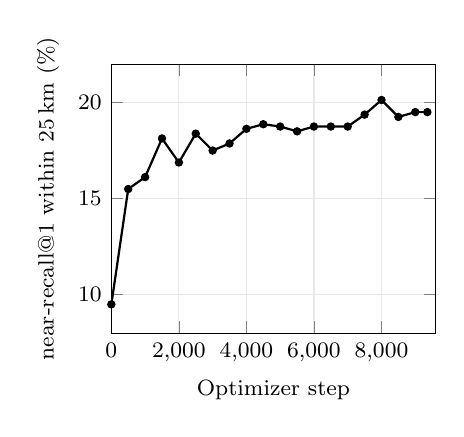
\begin{tikzpicture}
\begin{axis}[
  width=0.47\textwidth, height=5.0cm,
  xlabel={Optimizer step}, ylabel={near-recall@1 within 25\,km (\%)},
  xmin=0, xmax=9600, ymin=8, ymax=22,
  grid=major, grid style={gray!18},
  tick label style={font=\footnotesize}, label style={font=\footnotesize},
]
\addplot[thick, black, mark=*, mark size=1.1pt] coordinates {
(0,9.50) (500,15.50) (1000,16.12) (1500,18.13) (2000,16.88) (2500,18.38) (3000,17.50)
(3500,17.87) (4000,18.63) (4500,18.87) (5000,18.75) (5500,18.50) (6000,18.75) (6500,18.75)
(7000,18.75) (7500,19.37) (8000,20.13) (8500,19.25) (9000,19.50) (9358,19.50)};
\end{axis}
\end{tikzpicture}
\hfill
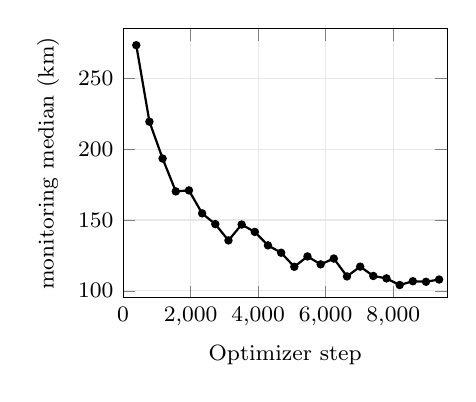
\begin{tikzpicture}
\begin{axis}[
  width=0.47\textwidth, height=5.0cm,
  xlabel={Optimizer step}, ylabel={monitoring median (km)},
  xmin=0, xmax=9600, ymin=95, ymax=285,
  grid=major, grid style={gray!18},
  tick label style={font=\footnotesize}, label style={font=\footnotesize},
]
\addplot[thick, black, mark=*, mark size=1.1pt] coordinates {
(390,273.4) (780,219.4) (1170,193.4) (1560,170.2) (1950,170.9) (2340,154.7) (2730,147.1)
(3120,135.6) (3510,146.8) (3900,141.6) (4290,132.1) (4680,126.9) (5070,117.0) (5460,124.3)
(5850,118.7) (6240,122.8) (6630,110.2) (7020,117.1) (7410,110.5) (7800,108.8) (8190,104.1)
(8580,106.8) (8970,106.4) (9358,108.0)};
\end{axis}
\end{tikzpicture}
\caption{The from-scratch joint encoder, both objectives logged live over its single epoch.
Left: the held-out retrieval probe, which doubles from $9.5\%$ to $19.5\%$. Right: the
classifier's monitoring median, which reaches $104.1$~km, matching a three-epoch classifier
run in one joint epoch from scratch. Both curves say the recipe works. Its descriptors
nevertheless lose to the two warm-started encoders, which is the point of
Section~\ref{sec:attribution}.}
\label{fig:scratch}
\end{figure}

\section{Results}

\subsection{Main result}

\begin{table}[t]
\centering
\footnotesize
\begin{tabular}{lrrrrr}
\toprule
System & median (km) & @1~km & @25~km & @200~km & mean (km) \\
\midrule
\multicolumn{6}{l}{\emph{Reported on other evaluation sets, not directly comparable}} \\
PIGEON, single image \cite{haas2024pigeon} & 131 & $0.9\%$ & $24.2\%$ & -- & -- \\
PIGEON, four-view panorama \cite{haas2024pigeon} & 44.4 & $5.4\%$ & $40.4\%$ & -- & -- \\
\midrule
\multicolumn{6}{l}{\emph{This work, all on the same frozen 2{,}998-image split}} \\
Prior system, full fine-tune, same corpus & 194 & -- & -- & -- & -- \\
Classifier stage only & 104.66 & $0.0\%$ & $7.6\%$ & $70.6\%$ & 456 \\
Full pipeline, $\lambda{=}1$ & 36.66 & $11.61\%$ & $45.86\%$ & -- & -- \\
\textbf{Full pipeline, $\lambda{=}2$} & \textbf{34.10} & $10.14\%$ & $\mathbf{46.26\%}$ & -- & 328 \\
On device, int8 index, 1 view per location & 44.4 & -- & $43.0\%$ & $73.9\%$ & -- \\
On device, int8 index, 4 views per location & 33.9 & -- & $46.4\%$ & $74.6\%$ & -- \\
\bottomrule
\end{tabular}
\caption{Headline results. The PIGEON rows are included for orientation only; they are
measured on a different held-out set and a different image distribution, and no claim of a
controlled comparison is made. The on-device rows are measured with the exact quantized
assets the application ships, on the same validation split.}
\label{tab:main}
\end{table}

The final system scores a median great-circle error of $34.10$~km, with $46.26\%$ of images
placed within 25~km and $10.14\%$ within 1~km, at a mean of $328$~km and a GeoGuessr score of
$4470$ per round. Table~\ref{tab:main} places this in context.

We include PIGEON's published numbers because it is the closest comparable system and because
they were the target we set ourselves, but they are measured on a different evaluation set,
and we make no claim of a controlled comparison. The internally controlled comparison is the
one against the same author's prior system, which used the identical $1.2$~M-image corpus with
a full backbone fine-tune and scored $194$~km. Against that, with $5\%$ of the trainable
parameters, the classifier stage alone is $46\%$ better and the full pipeline is $82\%$
better.

\subsection{Stage-by-stage ablation}

\begin{table}[t]
\centering
\footnotesize
\begin{tabular}{llrrrr}
\toprule
& Stage & median (km) & @1~km & @25~km & mean (km) \\
\midrule
(a) & Classifier, full corpus, 3 epochs & 104.66 & $0.0\%$ & $7.6\%$ & 456 \\
(b) & \quad $+$ retrieval: mass gate, cosine kNN, snap & 78.52 & $10.24\%$ & $35.16\%$ & -- \\
(c) & \quad $+$ tuned gate, prior $\lambda{=}0.05$, $k{=}1$ & 65.66 & $10.11\%$ & $35.99\%$ & -- \\
(d) & \quad $+$ contrastive place head, cached vectors & 61.16 & $11.47\%$ & $38.69\%$ & 390 \\
(e) & \quad $+$ geo-smooth positives, two-head blend & 49.04 & $11.57\%$ & $41.16\%$ & 388 \\
(f) & \quad $+$ mean-patch descriptor, chamfer rerank & 43.75 & $11.27\%$ & $42.93\%$ & 373 \\
(g) & \quad $+$ contrastive encoder, bands, CSLS, whitening & 36.96 & $12.78\%$ & $46.06\%$ & 378 \\
(h) & \quad $+$ joint encoder, learned reranker ($\lambda{=}2$) & \textbf{34.10} & $10.14\%$ & $\mathbf{46.26\%}$ & \textbf{328} \\
\bottomrule
\end{tabular}
\caption{The full progression on the frozen validation split. Rows (b) through (h) are
inference-time only with respect to the classifier: it has not been retrained since row (a).
Rows (b) to (g) cost approximately \$6 of rented GPU time in aggregate; row (h)'s reranker
cost nothing beyond CPU minutes. The chain is cumulative with one exception: the
configuration in row (h) retires the chamfer rerank introduced in row (f), whose benefit no
longer justified its cost once the learned reranker was in place.}
\label{tab:progression}
\end{table}

Table~\ref{tab:progression} gives the complete progression. The shape of it is the argument of
this paper: the largest single jump, $104.66 \rightarrow 78.52$~km, comes from reusing already
computed features as a retrieval index, with no training at all.

\subsection{Encoder attribution}
\label{sec:attribution}

\begin{table}[t]
\centering
\small
\begin{tabular}{lrrrr}
\toprule
& \multicolumn{2}{c}{recipe only} & \multicolumn{2}{c}{$+$ learned reranker} \\
\cmidrule(lr){2-3}\cmidrule(lr){4-5}
Encoder behind the index & median (km) & @25~km & median (km) & @25~km \\
\midrule
None: frozen classifier features & 49.04 & $41.16\%$ & 42.74 & $43.1\%$ \\
Contrastive, warm-started & \textbf{36.96} & $\mathbf{46.06\%}$ & not measured & -- \\
Joint with graded targets, warm-started & 40.98 & $44.13\%$ & \textbf{34.10} & $\mathbf{46.26\%}$ \\
Joint, from scratch, one epoch & 47.82 & $42.56\%$ & 38.65 & $45.10\%$ \\
\bottomrule
\end{tabular}
\caption{The four indices compared at a matched post-processing recipe (band blend, hubness
correction, whitening), and again with the learned reranker on top. The reranker figures use
$\lambda = 1$ for the frozen-feature index and $\lambda = 2$ for the other two. The champion
configuration is the jointly trained encoder plus the reranker, even though that encoder's
descriptors are worse than the purely contrastive one's at matched recipe.}
\label{tab:encoders}
\end{table}

Table~\ref{tab:encoders} is the table we would most like other people to copy, because it makes an
uncomfortable attribution explicit. Our champion configuration uses the jointly trained
encoder, but that encoder's descriptors are \emph{worse} than the purely contrastive one's
under an identical recipe, $40.98$ against $36.96$~km. It became the champion because it is
the index the reranker happened to be fit and evaluated on, and the reranker is worth more
than the difference between the two encoders. The correct reading is that the $34.10$~km
result is the reranker's win, not the encoder's.

One cell of the table is missing, and it is the one we most regret. The purely contrastive
index, the best of the four under the matched recipe, never received the reranker: its
cached candidate pools were lost with the machine that produced them, before the reranker
existed. Regenerating them costs a few dollars, and doing so is the first measurement anyone
extending this work should take, because it could plausibly beat $34.10$.

The from-scratch encoder is a cleaner negative, and the more interesting one, because it
succeeded at everything it was measured on during training and still lost. In a single joint
epoch its held-out retrieval probe doubled, from $9.5\%$ to $19.5\%$ near-recall within
25~km, and its classifier reached $104.1$~km, matching a three-epoch classifier run
(Figure~\ref{fig:scratch}). Its descriptors nevertheless lose to both warm-started encoders,
which carry roughly three and a half epochs of accumulated backbone adaptation between them.
A corroborating diagnostic: its descriptor space has a mean hubness statistic of $0.787$
against the joint encoder's $0.604$, that is, it is measurably under-differentiated, with more
of the index acting as a nearest neighbour to everything. The conclusion is narrow but useful:
one joint epoch from scratch is enough to match the classifier and not enough to match the
descriptors, so the two objectives converge at different rates on the same backbone.

\subsection{Where the remaining error lives}
\label{sec:ceilings}

Three ceilings, all measured on the same validation split, decompose the residual error and
close off three directions.

\textbf{Coverage is $100\%$.} For every single validation image there exists a training image
within 25~km, and the median nearest training image is $2.2$~km away, with $38.5\%$ of queries
having a training image within 1~km. More data cannot raise this ceiling, though denser
coverage would still make the matcher's task easier. This was measured before any
retrieval work began and is what justified the entire second stage.

\textbf{In-pool oracle is $92$ to $98\%$.} Restricted to the candidates the gate actually
shows, a perfect matcher would place $92\%$ of queries within 25~km at a mass threshold of
$0.8$ and $97.6\%$ at $0.95$. The gate is not the constraint either.

\textbf{The matcher converts $46\%$.} That is the number we actually achieve.

So approximately fifty percentage points of $\mathrm{acc@}25$ sit entirely in matching
quality. Not in coverage, not in the gate, not in the cell scheme. Two full rounds of head
engineering moved it from $38.7$ to $42.9\%$ with sharply diminishing returns, which is the
evidence that the limit lies in the features themselves. A backbone tuned to tell Finland from
Canada keeps what distinguishes Finland from Canada and discards what distinguishes one
Finnish road from the next.

There is a further arithmetic consequence worth stating, because it sets the target for
whoever continues this. The moment $\mathrm{acc@}25$ crosses $50\%$, the median is
mathematically below 25~km. One lever moves both metrics.

\subsection{Distance profile}

\begin{table}[t]
\centering
\small
\begin{tabular}{lr@{\hskip 2.5em}lr@{\hskip 2.5em}lr}
\toprule
within & share & within & share & percentile & error \\
\midrule
100~m & $2.97\%$ & 50~km & $51.83\%$ & p10 & 0.8~km \\
500~m & $7.74\%$ & 200~km & $73.92\%$ & p25 & 5.4~km \\
1~km & $11.27\%$ & 1000~km & $94.50\%$ & p50 & 43.8~km \\
5~km & $24.15\%$ & & & p75 & 211~km \\
10~km & $31.72\%$ & & & p90 & 564~km \\
25~km & $42.93\%$ & & & p99 & 7986~km \\
\bottomrule
\end{tabular}
\caption{Full distance profile at the multi-descriptor stage, median $43.75$~km, on all 2{,}998 validation
images. We report the profile at this stage because it is the configuration for which the
complete per-image distance array was archived. The GeoGuessr score at this configuration is
$4438$ per round, $4856$ median round, $22{,}188$ per five-round game, with $69.3\%$ of rounds
above $4500$.}
\label{tab:profile}
\end{table}

Table~\ref{tab:profile} gives the shape of the error distribution. The distribution is
strikingly bimodal in practical terms. A quarter of all queries land within $5.4$~km, which is
usable-street-level accuracy, and one query in a hundred lands nearly eight thousand
kilometres away. There is very little in between, and this is why the mean is a poor summary
and the median a good one.

\subsection{External benchmarks: transfer to consumer photographs}
\label{sec:external}

Every number so far is measured on held-out Street View imagery. To measure transfer to
consumer photographs directly, we ran the frozen champion pipeline on the two standard
benchmarks of the field: IM2GPS \cite{hays2008im2gps} (237 Flickr images) and IM2GPS3k
\cite{vo2017revisiting} (2{,}997 Flickr images). The protocol involves no benchmark-side
fitting of any kind: the encoder, gate, blend weights, hubness correction, whitening and the
E7 reranker (fit once on our own validation split) are all applied exactly as deployed.

\begin{table}[t]
\centering
\footnotesize
\setlength{\tabcolsep}{4pt}
\begin{tabular}{lrrrrrl}
\toprule
System & @1~km & @25~km & @200~km & @750~km & @2500~km & training imagery \\
\midrule
ISNs \cite{mullerbudack2018geolocation} & $10.5$ & $28.0$ & $36.6$ & $49.7$ & $66.0$ & 4.7M Flickr \\
GeoCLIP \cite{cepeda2023geoclip} & $14.1$ & $34.5$ & $50.7$ & $69.7$ & $83.8$ & 4.7M Flickr \\
PIGEOTTO \cite{haas2024pigeon} & $11.3$ & $36.7$ & $53.8$ & $72.4$ & $85.3$ & 4.5M Flickr+landmarks \\
\midrule
Ours, classifier argmax & $0.0$ & $3.2$ & $17.4$ & $38.0$ & $60.7$ & 1.2M Street View \\
Ours, full pipeline & $0.5$ & $9.6$ & $20.3$ & $41.2$ & $65.0$ & 1.2M Street View \\
\midrule
Oracle: nearest index image & $13.6$ & $86.8$ & $90.6$ & $98.3$ & $100.0$ & (index coverage bound) \\
\bottomrule
\end{tabular}
\caption{IM2GPS3k, percentage of queries localized within each radius. Published rows are
from the cited papers; all are trained on Flickr-distribution corpora, the same distribution
the benchmark is drawn from. The oracle row is the fraction of queries for which \emph{any}
index image lies within the radius: the ceiling of any retrieval over our index.}
\label{tab:im2gps3k}
\end{table}

Table~\ref{tab:im2gps3k} reports IM2GPS3k; IM2GPS is qualitatively identical (median
$660$~km, $10.1\%$ at 25~km). The result is poor, and the decomposition says precisely why.
Index coverage is not the bottleneck at city scale: an index image within 25~km exists for
$86.8\%$ of IM2GPS3k queries. But the matcher converts that coverage $11\%$ of the time,
against $46\%$ in-domain. A Street View--trained descriptor is being asked to match a
Flickr close-up, an indoor scene or a landmark photograph against road-level views of the
same place, and mostly cannot. At street scale the index itself caps the task: only $13.6\%$
of queries have \emph{any} index image within 1~km, so even a perfect matcher could not
reach GeoCLIP's $14.1\%$. Two facts survive the transfer intact. Retrieval still triples the
classifier ($3.2\% \to 9.6\%$ at 25~km, median $1498 \to 1144$~km), so the structural claim
of this paper, classify to look and retrieve to answer, holds out of domain. And the
failure is a corpus property rather than a method property: the published systems above
train on the benchmark's own distribution, while the two Street View--trained systems in the
literature simply do not report these benchmarks (PIGEON proper was never evaluated on them,
and OSV-5M \cite{astruc2024osv5m} declines the comparison, judging roughly a third of
IM2GPS3k non-localizable). We report the numbers anyway: they are the honest measurement of
the domain gap that Section~\ref{sec:limitations} previously only asserted.

\section{Negative results}
\label{sec:negatives}

The ledger contains thirty-five rejected ideas. We group the informative ones.

\paragraph{Auxiliary classification heads improve every diagnostic and not the objective.}
Geo-contrastive hard negatives, a per-cell prototype cosine head, a surgical rerank in which
a fused score selects cells while the original posterior weights the spherical mean, and an
exponential moving average of the trainables were each tried. Every one of them raised cell
top-1 and top-5 accuracy, in one case to the best values recorded in the whole program, and
every one left the median flat or worse. The lesson generalizes: cell top-1 is a pessimistic
proxy for a median objective, because a one-point gain in top-1 moves too few validation rows
to shift the fiftieth percentile. We stopped proposing ideas in this family after the fourth
independent confirmation.

\paragraph{Within-cell refinement fails while cell selection is bad.} A per-cell
tangent-plane offset regression head, evaluated twice under different parameterizations, and
a barycentric soft-label scheme designed to be exactly invertible by the readout, both lost.
At a cell top-1 of $18\%$, regressing position inside a 250~km cell is about as hard as the
classification itself, and refining within a cell that is usually the wrong cell cannot help.
This directly contradicts the OSV-5M \cite{astruc2024osv5m} finding at their scale, and we
believe the reconciliation is simply that classify-then-regress requires a converged selector.

\paragraph{Query-side augmentation is dead in retrieval.} Test-time augmentation with three
centre crops cost $9.3$~km on the classifier. Query-side flips and zooms cost $0.4$
percentage points of $\mathrm{acc@}25$. A multi-resolution ensemble combining the $512$~px and
$384$~px indices of the \emph{same} model cost $0.9$ points, because the same model's errors
at two resolutions are correlated and there is no diversity to exploit. Database-side
augmentation remains untested and is the asymmetric version we would try next.

\paragraph{Batch samplers that reduce location diversity are catastrophic.} A panorama InfoNCE
auxiliary using same-panorama pair batches cost $23$~km. A distillation scheme grouping four
views per location cost $30$~km. An online confusion-driven sampler upweighting confused
country pairs cost $7$~km. Three independent confirmations of the same law: at a fixed step
budget, distinct locations per batch is the scarce resource, and any sampler that spends it
loses more than the auxiliary signal returns.

\paragraph{Classical retrieval post-processing does not transfer.} We implemented
$k$-reciprocal re-ranking \cite{zhong2017reranking} in two fair variants, visual and
geographic graph diffusion, and SuperGlobal-style query expansion \cite{shao2023superglobal}
in two variants. All were neutral or negative. Our reading is that these methods assume a
database in which true matches form dense mutual neighbourhoods, whereas a worldwide Street
View index is dominated by generic scenes for which that assumption fails.

\paragraph{No post-hoc decision rule can fix the mean.} This is the most decisive negative
result in the project and it took six experiments to establish. The mean is owned by roughly
$5\%$ of queries where both evidence channels, the descriptor space and the classifier
posterior, point confidently at the wrong region. We tried falling back to the classifier
(twice, the second time with corrected centroids), jumping to the training-density prior,
shrinking toward the prior, snapping to a geometric median, and re-gating at mass $0.995$ for
low-confidence queries. All failed, and they failed for a reason that generalizes: the
outcome-selected tail is not the detector-selected tail. Queries the system is uncertain about
are ones it already handles decently, whereas the truly catastrophic misses are
\emph{confidently} wrong, so no confidence threshold isolates them. Progress on the mean
requires new evidence channels, not new arithmetic on the existing ones.

\paragraph{Miscellaneous closed questions.} The smoothing temperature $\tau$ was swept at
40, 75 and 110~km and closed at 75. The cell count was swept at 512, 2048, 4096 and
5000, and at the experimental budget closed at 2048. Learning rates were
swept and closed. LoRA rank 32 lost to rank 16, because capacity costs steps. A hexagonal
balanced tessellation classified far better, top-1 $25.7\%$ against $18\%$, and guessed far
worse, $+26.5$~km, which is the quantization floor made visible. Muon \cite{jordan2024muon}
on the head matrices at learning rate $0.02$ lost by $26$~km, which we read as a
hyperparameter failure rather than a statement about the optimizer.

\section{Deployment}

The pipeline runs entirely offline on an Android phone. Nothing about the deployment is a
demonstration harness: it is the same encoder, the same gate, the same blend, the same CSLS
correction and the same reranker, ported to Kotlin and verified against the Python reference
on identical inputs, with 32 of 32 test images producing an identical top-1 match at a maximum
divergence of $0.000$~km.

\subsection{Accuracy and cost of quantization}

Two index configurations ship. A one-view-per-location index of $1.55$~GB scores $44.4$~km
median and $43.0\%$ within 25~km. A four-view index of $6.18$~GB scores $33.9$~km and
$46.4\%$. The four-view figure matches the research pipeline's own $34.10$~km, which means
int8 compression of the \emph{index} costs nothing measurable: the entire gap between the two
configurations is the three missing views per location, not the quantization.

\subsection{Massive activations make int8 unusable for this encoder}

Quantizing the \emph{encoder} is a completely different story, and the finding is worth
recording because it is not specific to this application. DINOv3 ViT-L carries a
massive-activation channel in its residual stream, peaking around $157{,}000$, of the kind
documented in large language models \cite{sun2024massive,dettmers2022llmint8}. Per-tensor
dynamic int8 quantization collapses the cosine similarity between the on-device descriptor
and the index descriptor from $0.989$ to $0.596$, and in the whitened space to $0.12$. The
same outlier overflows fp16 and yields NaN under a naive half-precision export.

The export that works stores all 156 linear layers in fp16 while keeping the LayerNorms, the
residual path and the patch-embedding convolution in fp32. This is numerically identical to
fp32 at half the size, $652$~MB against $1.3$~GB, and is what ships.

\subsection{Latency}

\begin{table}[t]
\centering
\small
\begin{tabular}{lrrr}
\toprule
& Pixel 10 Pro XL & Galaxy S21+ & S21+ thermally throttled \\
\midrule
Encode & 3.7~s & 6.4~s & 14.9~s \\
Search, one-view index & 156~ms & 470~ms & 750~ms \\
Startup & 1.1~s & 1.7~s & 7.8~s \\
\bottomrule
\end{tabular}
\caption{On-device latency, with search measured on the one-view index of 299{,}518
vectors. Retrieval is not the bottleneck; the ViT-L forward pass is, and it
scales directly with sustained CPU clock.}
\label{tab:latency}
\end{table}

Table~\ref{tab:latency} makes the engineering point plainly: searching the one-view index
costs $156$~ms and encoding one image costs $3.7$~s. The four-view index multiplies the
search term by four at most, which changes nothing about the balance. Retrieval, the
component that produces almost all of the accuracy, is essentially free at this scale, and
the entire latency budget belongs to the backbone. The throttled column is instructive: sustained inference heat-soaks
an Exynos 2100 from $2912$ to $533$~MHz, and every number degrades by that same factor, which
is a useful reminder that on-device benchmarks without a thermal column are not benchmarks.

One implementation detail cost a day and is worth passing on. The
\texttt{createScaledBitmap} call on Android is bilinear, while the index was built with
Pillow's bicubic resampler. The resulting descriptor drift is small in pixel terms and large in
retrieval terms. The shipped preprocessing reimplements Pillow's bicubic resampler by hand.

\section{Discussion}

\subsection{Why retrieval wins here}

The result admits a compact explanation. A classifier over $N$ cells has an output space of
size $N$; its predictions are, up to the interpolation the soft readout provides, confined to
$N$ points on a sphere. A retrieval system's output space is the set of training coordinates,
which here has $299{,}518$ distinct elements covering every validation query to within
$2.2$~km on the median. The second output space is simply much better matched to a
kilometre-scale objective, and no amount of classifier improvement changes that.

What the classifier is genuinely good at is deciding where to look. Its posterior, gated at
$95\%$ mass, reduces $1.2$~M candidates to about $22{,}000$ while retaining a within-25~km
candidate $92$ to $98\%$ of the time. That is an excellent instrument, and it is exactly the
instrument that a pure retrieval system lacks.

\subsection{The economics of cached-vector research}

A theme that runs through the whole project is that experiments on cached vectors cost cents while
experiments involving images cost dollars, and the ratio is roughly three orders of magnitude.
The entire progression from $104.7$ to $36.96$~km cost approximately \$9 of rented GPU time.
The reranker that took it to $34.10$~km cost nothing but CPU minutes on a laptop.

This suggests an operating discipline that we came to late and would adopt from the start next
time: the product of a run on rented hardware is not a model, it is a cache. The complete set
of artifacts, descriptors for both splits, logits, the gated candidate list per query,
candidate pools for reranker training, attribute posteriors, is what allows every subsequent
experiment to run on a CPU in minutes. The last of our encoder runs was designed explicitly
around that contract, with a manifest checked before the machine was allowed to be destroyed.
The encoder it produced lost. The cache it produced is still being used.

\subsection{Limitations}
\label{sec:limitations}

The headline evaluation is on a single held-out split of one Street View corpus, and Street
View imagery has a distinctive and consistent capture process. Section~\ref{sec:external}
now measures transfer to consumer photographs directly, and the measurement is sobering:
$9.6\%$ at 25~km on IM2GPS3k against $34$--$37\%$ for Flickr-trained systems. The
decomposition there shows the gap is dominated by descriptor domain shift rather than index
coverage, which bounds what any amount of post-hoc lever-pulling on the current corpus can
recover. Closing it requires consumer-distribution imagery in both the fine-tune and the
index; it is a data problem before it is a method problem.

The reranker is fit and evaluated by cross-validation on the same 2{,}998 queries. The folds
are disjoint by query and no query is scored by a model that saw it, so the numbers are not
optimistically biased in the usual sense, but the feature set and the blending weight
$\lambda$ were selected with knowledge of this split. We would not defend the third
significant figure of $34.10$.

The mean, at $328$~km, is not good, and Section~\ref{sec:negatives} explains why we believe no
rearrangement of the current evidence will improve it. The system fails confidently, which is
the worst failure mode for a user-facing product, and a genuine confidence estimate remains
unsolved.

Finally, our comparison to published systems is uncontrolled. Different evaluation sets,
different image distributions. We have been careful to label it as orientation rather than
as a result.

\subsection{Privacy}

A system that turns an arbitrary photograph into coordinates is useful and abusable in
equal measure: the capability that lets a hiker identify a trailhead also lets a stranger
narrow down a home from a shared snapshot. The authors of PIGEON \cite{haas2024pigeon}
discuss this tension at length and chose not to release their strongest model, and we take
their reasoning seriously. For privacy purposes the honest summary of our system is not the
median but the tail of Table~\ref{tab:profile}: roughly one photograph in ten resolves to
within a kilometre of where it was taken, and that is the number a release decision should
weigh. Two further facts bear on such a decision. The deployed pipeline runs entirely
offline, so no safeguard can be added on a server after the fact. And the index derives
from Street View imagery, so any redistribution is bounded by the licensing terms of the
source imagery rather than by ours.

\subsection{Notes on autonomous experimentation}

Three observations from running a research program this way.

The frozen evaluator is not a formality. It is the only thing that makes an autonomous agent's
self-reported results trustworthy, and enforcing it structurally, by uploading only the
mutable artifact to the compute node, is much stronger than enforcing it by instruction.

The negative record is the expensive artifact. An agent that does not remember its rejections
re-proposes them, and the accumulated dead-end list was consulted more
often than the champion configuration. We would now design the log format before designing the
loop.

Instrument the training loop with the metric the final decision uses. Our contrastive fine-tune ran
blind for 42 minutes: its contrastive loss swings by a factor of two purely on the geographic
difficulty of the sampled region and therefore forecasts nothing, and its five intermediate
checkpoints could not be ranked without a full re-index each. A two-second held-out retrieval
probe would have provided both a forecast and a checkpoint selection criterion. We added one
before every subsequent run.

\subsection{Future work}

The ceiling analysis in Section~\ref{sec:ceilings} points at exactly one target: within-pool
matching quality, currently $46\%$ against an oracle of $92$ to $98\%$. Three directions
follow directly. Replacing CLS pooling with an optimal-transport aggregation over patch tokens
\cite{izquierdo2024salad} is the largest literature-endorsed descriptor gain available and we
already compute and discard the necessary patch tokens. Geometric verification of the top ten
candidates \cite{hausler2021patchnetvlad} attacks perceptual aliasing directly, since true
neighbours share scene geometry while 300~km lookalikes share only statistics. And the
reranker should be scaled: the version reported here is a sixteen-feature logistic fit on
three thousand queries, and a train-side episode cache of $1.2$~M mined pools already exists
for fitting a much larger one with a graded rather than binary target.

For the mean, the direction is new evidence channels rather than new decision rules:
attribute probes over free coordinate-derived labels used as inference-time constraints on the
gate, and a script-identification or OCR channel, which is high-precision where it fires.

\section{Conclusion}

We set out to place a single photograph on the globe and reached a median error of $34.1$~km,
with the whole system running offline on a phone. The result was obtained by treating a
geocell classifier as a search-space reducer rather than as a predictor, and by spending
almost all of the remaining effort on cheap operations over cached vectors: contrastive
projections fit offline, hubness correction, whitening, and a small learned reranker whose
most valuable features measure geographic consensus among candidates rather than visual
similarity to the query.

The measurement we would most like to be remembered is the ceiling decomposition. Coverage is
perfect, the gate is nearly perfect, and the matcher converts less than half of what it is
handed. Everything that matters in this problem, at this accuracy level, is in the matcher.

\section*{Acknowledgements}

The experimental loop is a fork of \texttt{karpathy/autoresearch}
\cite{karpathy2026autoresearch}, whose keep-or-reset design and frozen-harness discipline are
the reason the ledger in this paper is trustworthy. All experiments were proposed, implemented
and executed by an autonomous agent under human supervision; the author set the objective,
approved spending, and vetoed on grounds the metric could not see.

\begin{thebibliography}{99}
\small

\bibitem{alibey2024boq}
A.~Ali-bey, B.~Chaib-draa, and P.~Gigu\`ere.
\newblock BoQ: A place is worth a bag of learnable queries.
\newblock In \emph{CVPR}, 2024.

\bibitem{arandjelovic2016netvlad}
R.~Arandjelovi\'c, P.~Gron\'at, A.~Torii, T.~Pajdla, and J.~Sivic.
\newblock NetVLAD: CNN architecture for weakly supervised place recognition.
\newblock In \emph{CVPR}, 2016.

\bibitem{astruc2024osv5m}
G.~Astruc, N.~Dufour, I.~Siglidis, C.~Aronssohn, N.~Bouia, S.~Fu, R.~Loiseau, V.~N.~Nguyen,
C.~Raude, E.~Vincent, L.~Xu, H.~Zhou, and L.~Landrieu.
\newblock OpenStreetView-5M: The many roads to global visual geolocation.
\newblock In \emph{CVPR}, 2024.

\bibitem{berton2022rethinking}
G.~Berton, C.~Masone, and B.~Caputo.
\newblock Rethinking visual geo-localization for large-scale applications.
\newblock In \emph{CVPR}, 2022.

\bibitem{berton2023eigenplaces}
G.~Berton, G.~Trivigno, B.~Caputo, and C.~Masone.
\newblock EigenPlaces: Training viewpoint robust models for visual place recognition.
\newblock In \emph{ICCV}, 2023.

\bibitem{cepeda2023geoclip}
V.~Vivanco~Cepeda, G.~K.~Nayak, and M.~Shah.
\newblock GeoCLIP: Clip-inspired alignment between locations and images for effective
worldwide geo-localization.
\newblock In \emph{NeurIPS}, 2023.

\bibitem{semivariogram2025}
B.~Chen, Z.~Wang, F.~Deuser, J.~M.~Zollner, and M.~Werner.
\newblock Enhancing contrastive learning for geolocalization by discovering hard negatives
on semivariograms.
\newblock arXiv:2509.21573, 2025.

\bibitem{chen2020simple}
T.~Chen, S.~Kornblith, M.~Norouzi, and G.~Hinton.
\newblock A simple framework for contrastive learning of visual representations.
\newblock In \emph{ICML}, 2020.

\bibitem{pinpoint2026}
N.~Chuzhoy, B.~Hu, A.~A.~Arora, J.~Ro, and S.~S.~Sahu.
\newblock Pinpoint: Grounded worldwide image geolocation via cross-source retrieval and
reranking.
\newblock arXiv:2606.04133, 2026.

\bibitem{clark2023where}
B.~Clark, A.~Kerrigan, P.~P.~Kulkarni, V.~V.~Cepeda, and M.~Shah.
\newblock Where we are and what we're looking at: Query based worldwide image geo-localization
using hierarchies and scenes.
\newblock In \emph{CVPR}, 2023.

\bibitem{conneau2018word}
A.~Conneau, G.~Lample, M.~Ranzato, L.~Denoyer, and H.~J\'egou.
\newblock Word translation without parallel data.
\newblock In \emph{ICLR}, 2018.

\bibitem{dettmers2022llmint8}
T.~Dettmers, M.~Lewis, Y.~Belkada, and L.~Zettlemoyer.
\newblock LLM.int8(): 8-bit matrix multiplication for transformers at scale.
\newblock In \emph{NeurIPS}, 2022.

\bibitem{dosovitskiy2021image}
A.~Dosovitskiy, L.~Beyer, A.~Kolesnikov, D.~Weissenborn, X.~Zhai, T.~Unterthiner,
M.~Dehghani, M.~Minderer, G.~Heigold, S.~Gelly, J.~Uszkoreit, and N.~Houlsby.
\newblock An image is worth 16x16 words: Transformers for image recognition at scale.
\newblock In \emph{ICLR}, 2021.

\bibitem{hierloc2026}
H.~K.~Gadi, D.~Matos, H.~Luo, L.~Liu, Y.~Wang, Y.~Zhang, and L.~Meng.
\newblock HierLoc: Hyperbolic entity embeddings for hierarchical visual geolocation.
\newblock In \emph{ICLR}, 2026.

\bibitem{geman1987statistical}
S.~Geman and D.~E.~McClure.
\newblock Statistical methods for tomographic image reconstruction.
\newblock \emph{Bulletin of the International Statistical Institute}, 52:5--21, 1987.

\bibitem{haas2024pigeon}
L.~Haas, M.~Skreta, S.~Alberti, and C.~Finn.
\newblock PIGEON: Predicting image geolocations.
\newblock In \emph{CVPR}, 2024.

\bibitem{hausler2021patchnetvlad}
S.~Hausler, S.~Garg, M.~Xu, M.~Milford, and T.~Fischer.
\newblock Patch-NetVLAD: Multi-scale fusion of locally-global descriptors for place
recognition.
\newblock In \emph{CVPR}, 2021.

\bibitem{hays2008im2gps}
J.~Hays and A.~A.~Efros.
\newblock IM2GPS: Estimating geographic information from a single image.
\newblock In \emph{CVPR}, 2008.

\bibitem{hu2022lora}
E.~J.~Hu, Y.~Shen, P.~Wallis, Z.~Allen-Zhu, Y.~Li, S.~Wang, L.~Wang, and W.~Chen.
\newblock LoRA: Low-rank adaptation of large language models.
\newblock In \emph{ICLR}, 2022.

\bibitem{izquierdo2024salad}
S.~Izquierdo and J.~Civera.
\newblock Optimal transport aggregation for visual place recognition.
\newblock In \emph{CVPR}, 2024.

\bibitem{jegou2012negative}
H.~J\'egou and O.~Chum.
\newblock Negative evidences and co-occurrences in image retrieval: The benefit of PCA and
whitening.
\newblock In \emph{ECCV}, 2012.

\bibitem{jordan2024muon}
K.~Jordan, Y.~Jin, V.~Boza, J.~You, F.~Cesista, L.~Newhouse, and J.~Bernstein.
\newblock Muon: An optimizer for hidden layers in neural networks.
\newblock Technical report, 2024.

\bibitem{karpathy2026autoresearch}
A.~Karpathy.
\newblock autoresearch: A minimal single-agent research ratchet.
\newblock \url{https://github.com/karpathy/autoresearch}, 2026.

\bibitem{liu2023patchdropout}
Y.~Liu, C.~Matsoukas, F.~Strand, H.~Azizpour, and K.~Smith.
\newblock PatchDropout: Economizing vision transformers using patch dropout.
\newblock In \emph{WACV}, 2023.

\bibitem{loshchilov2019decoupled}
I.~Loshchilov and F.~Hutter.
\newblock Decoupled weight decay regularization.
\newblock In \emph{ICLR}, 2019.

\bibitem{mullerbudack2018geolocation}
E.~M\"uller-Budack, K.~Pustu-Iren, and R.~Ewerth.
\newblock Geolocation estimation of photos using a hierarchical model and scene
classification.
\newblock In \emph{ECCV}, 2018.

\bibitem{oord2018representation}
A.~van~den~Oord, Y.~Li, and O.~Vinyals.
\newblock Representation learning with contrastive predictive coding.
\newblock arXiv:1807.03748, 2018.

\bibitem{oquab2024dinov2}
M.~Oquab, T.~Darcet, T.~Moutakanni, et~al.
\newblock DINOv2: Learning robust visual features without supervision.
\newblock \emph{Transactions on Machine Learning Research}, 2024.

\bibitem{radenovic2019finetuning}
F.~Radenovi\'c, G.~Tolias, and O.~Chum.
\newblock Fine-tuning CNN image retrieval with no human annotation.
\newblock \emph{IEEE TPAMI}, 41(7):1655--1668, 2019.

\bibitem{radovanovic2010hubs}
M.~Radovanovi\'c, A.~Nanopoulos, and M.~Ivanovi\'c.
\newblock Hubs in space: Popular nearest neighbors in high-dimensional data.
\newblock \emph{Journal of Machine Learning Research}, 11:2487--2531, 2010.

\bibitem{shao2023superglobal}
S.~Shao, K.~Chen, A.~Karpur, Q.~Cui, A.~Araujo, and B.~Cao.
\newblock Global features are all you need for image retrieval and reranking.
\newblock In \emph{ICCV}, 2023.

\bibitem{simeoni2025dinov3}
O.~Sim\'eoni, H.~V.~Vo, M.~Seitzer, et~al.
\newblock DINOv3.
\newblock arXiv:2508.10104, 2025.

\bibitem{su2024roformer}
J.~Su, M.~Ahmed, Y.~Lu, S.~Pan, W.~Bo, and Y.~Liu.
\newblock RoFormer: Enhanced transformer with rotary position embedding.
\newblock \emph{Neurocomputing}, 568:127063, 2024.

\bibitem{sun2018integral}
X.~Sun, B.~Xiao, F.~Wei, S.~Liang, and Y.~Wei.
\newblock Integral human pose regression.
\newblock In \emph{ECCV}, 2018.

\bibitem{sun2024massive}
M.~Sun, X.~Chen, J.~Z.~Kolter, and Z.~Liu.
\newblock Massive activations in large language models.
\newblock In \emph{COLM}, 2024.

\bibitem{tan2021instance}
F.~Tan, J.~Yuan, and V.~Ordonez.
\newblock Instance-level image retrieval using reranking transformers.
\newblock In \emph{ICCV}, 2021.

\bibitem{vo2017revisiting}
N.~Vo, N.~Jacobs, and J.~Hays.
\newblock Revisiting IM2GPS in the deep learning era.
\newblock In \emph{ICCV}, 2017.

\bibitem{weyand2016planet}
T.~Weyand, I.~Kostrikov, and J.~Philbin.
\newblock PlaNet: Photo geolocation with convolutional neural networks.
\newblock In \emph{ECCV}, 2016.

\bibitem{zhong2017reranking}
Z.~Zhong, L.~Zheng, D.~Cao, and S.~Li.
\newblock Re-ranking person re-identification with $k$-reciprocal encoding.
\newblock In \emph{CVPR}, 2017.

\end{thebibliography}

\appendix

\section{Experiment ledger summary}

The complete ledger is committed as a tab-separated file with one row per run, recording the
commit hash, the objective, peak memory, the verdict and a one-line diagnosis. Its summary
statistics are given in Table~\ref{tab:ledger}.

\begin{table}[h]
\centering
\small
\begin{tabular}{lr}
\toprule
Outcome & Runs \\
\midrule
Accepted (including baselines, machine anchors and confirmation re-runs) & 30 \\
Rejected & 35 \\
Crashed (out of memory, distributed deadlocks, scripted-edit bugs) & 9 \\
\midrule
Total logged & 74 \\
\bottomrule
\end{tabular}
\caption{Outcomes across the whole search phase. Crashes are logged because their
causes, memory pairing rules and collective-communication timeouts, are reusable knowledge.}
\label{tab:ledger}
\end{table}

Nine crashes is not a small number and we report it deliberately. Six were out-of-memory
failures, which established a standing rule that any memory-adding change must be paired with
a batch-size reduction in the same experiment. Two were distributed-training deadlocks caused
by running a diagnostic probe on all ranks, desynchronizing them past the collective timeout.
One was a scripted-edit bug that closed a class scope and silently removed a method, after
which every scripted edit to the model file was checked by parsing the resulting syntax tree.

\section{Reranker feature list}

For completeness, the sixteen per-candidate features of Section~\ref{sec:e7}, in order:
blended gated score; raw CLS cosine; $\log(1+\mathrm{rank})$; margin to the top candidate;
geographic consensus at 10, 25 and 50~km; one-step affinity diffusion of the score softmax;
affinity-weighted mean similarity to other candidates; mean of the three largest off-diagonal
affinities; pool entropy; pool fill fraction; and the four interactions of score, raw cosine,
margin and diffusion with the 25~km consensus term. Features are standardized across the
flattened candidate set. The softmax temperature is $0.05$, the affinity graph is thresholded
at cosine $0.5$ and row-normalized, and the logistic is fit by 400 steps of full-batch
gradient descent at learning rate $0.5$ under five-fold cross-validation over queries.

\section{Reproducibility}

The classifier, the retrieval engine, the offline head-training scripts, the lever sweeps and
the local evaluation scripts are all in the project repository, along with the research log,
the raw run ledger and the working notebooks. Checkpoints and cached descriptor arrays are
mirrored to a public model repository, folder per phase. The evaluator was never modified
during the study; the commit that introduced it predates every result in this paper.

Every run logged its full metric panel live to an experiment tracker, one run per experiment.
Figure~\ref{fig:ratchet} is plotted from the committed run ledger, and
Figures~\ref{fig:steps}, \ref{fig:fullruns} and \ref{fig:scratch} are plotted from the
tracker's recorded histories rather than redrawn by hand, so the curves are the ones the
decisions were actually made against. Where a figure shows the in-training monitoring
evaluation, which uses a 1{,}000-image subset, the corresponding full-split score is quoted
alongside it, because the two differ by a few kilometres and only the latter was ever used to
accept or reject a change.

\section{Parameter budget}

Table~\ref{tab:params} accounts for every parameter the final configuration trains. We include it
because the distribution is the argument of the paper in miniature: almost all of the accuracy
comes from the last two rows, and the last row has seventeen parameters.

\begin{table}[t]
\centering
\footnotesize
\begin{tabular}{llr}
\toprule
Component & Trained by & Parameters \\
\midrule
DINOv3 ViT-L/16 backbone & never & 300~M (frozen) \\
LoRA adapters, $r{=}16$, on $q,k,v,o$ & full run, then contrastive & 3.15~M \\
Trunk, fine heads A/B, coarse and country heads & full run & 12.0~M \\
Band place heads & offline, cached descriptors & 12.6~M \\
Learned reranker & offline, cached candidate pools, CPU & 17 \\
\midrule
Total trained & & 27.8~M ($9\%$) \\
\bottomrule
\end{tabular}
\caption{The complete parameter budget. The reranker, which is worth $6.9$~km of median error,
is a sixteen-weight logistic regression with a bias term.}
\label{tab:params}
\end{table}

\end{document}
